% DESCRIÇÃO DA IMPLEMENTAÇÃO-------------------------------------------------------------------

\chapter{DESCRIÇÃO DA IMPLEMENTAÇÃO}
\label{chap:descricao_da_implementacao}

Esse capítulo possui uma descrição completa de todas as partes do sistema. Cada uma delas foi separada em seu respectivo subcapítulo, possibilitanto uma melhor dissertação de todos os elementos que a compõe. Antes de iniciar essa abordagem aprofundada, deixamos um diagrama de como as partes do sistema estão interligadas.

\begin{figure}[!htb]
    \centering
    \caption{Diagrama da Arquitetura do Sistema}
    \frame{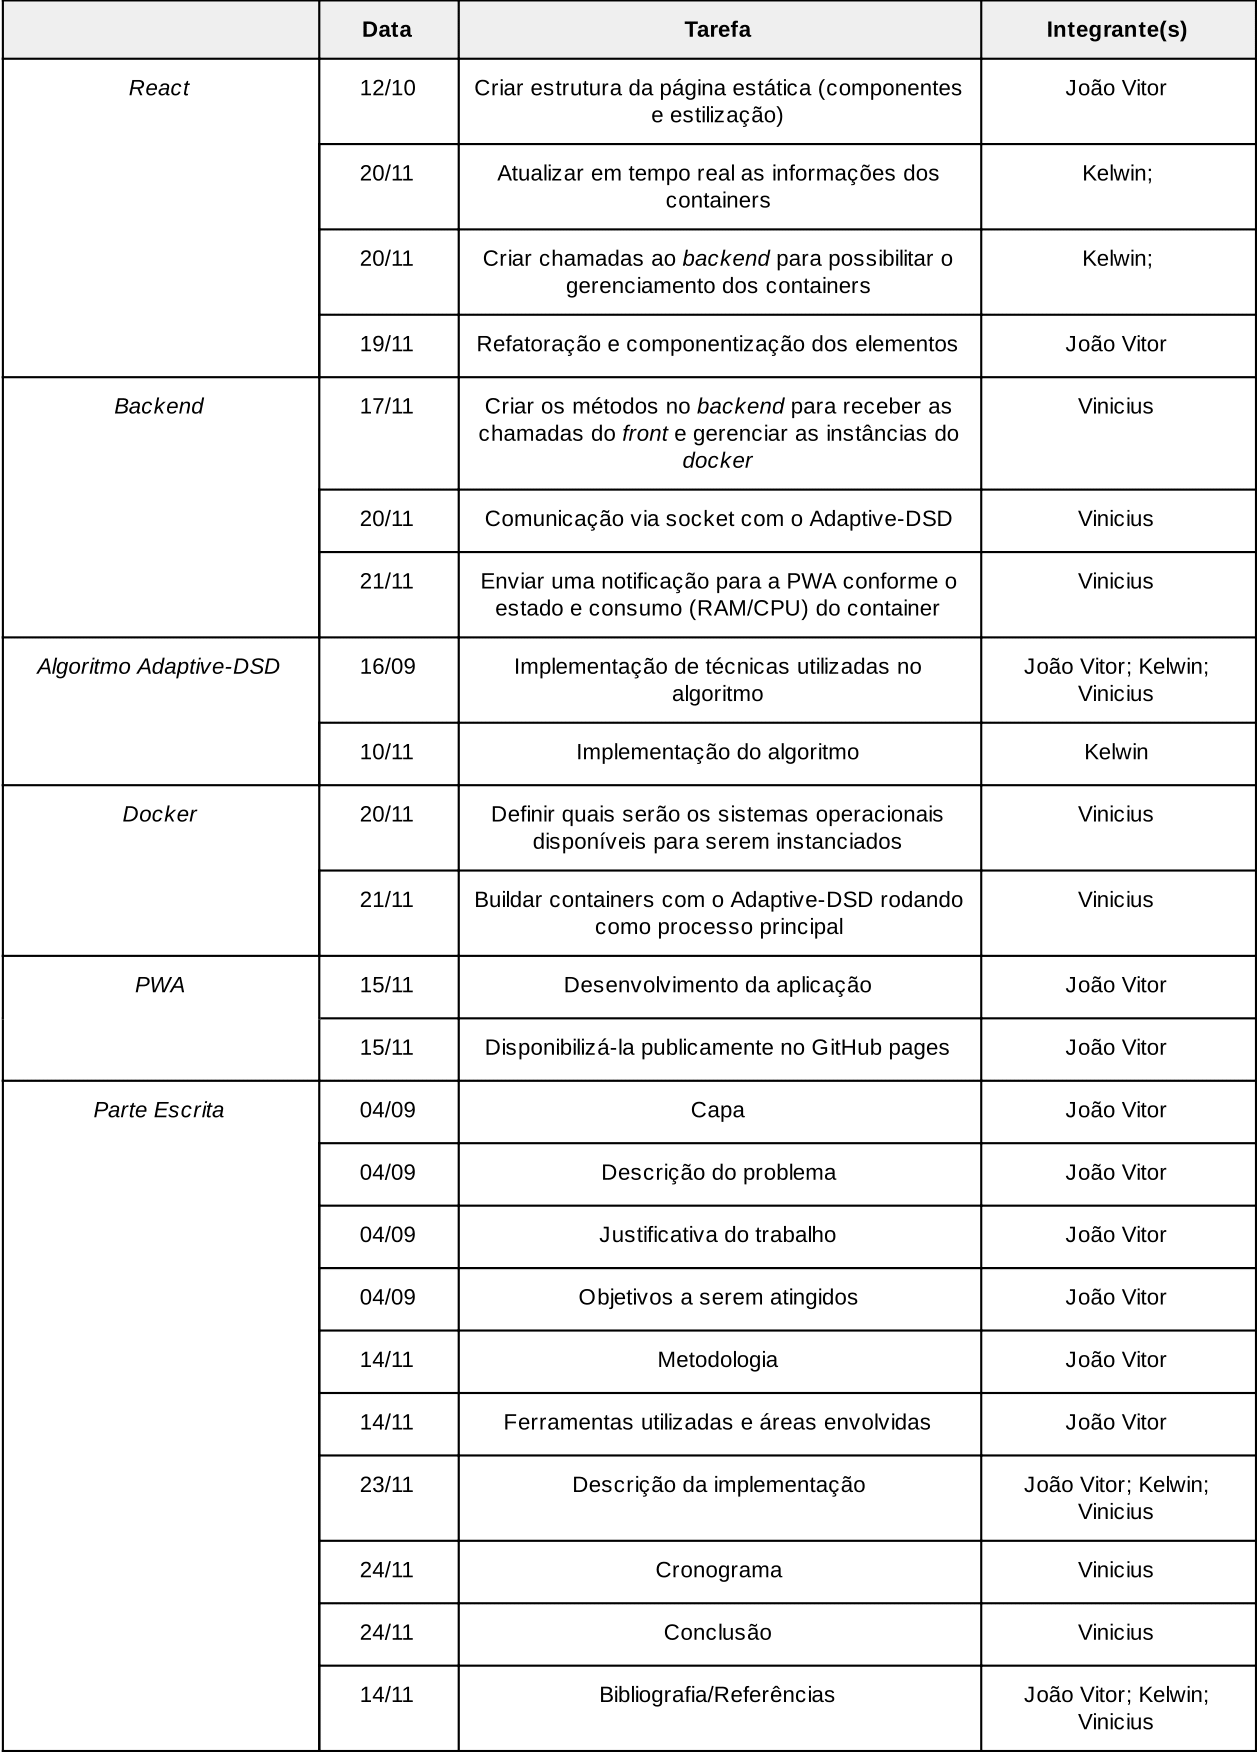
\includegraphics[width=1.0\textwidth]{./content/textuais/imagens/diagrama-arquitetura.png}}
    \label{fig:diagrama_arquitetura}
\end{figure}

% ADAPTIVE DSD-------------------------------------------------------------------
\section{\adaptive{}}
\label{sec:adaptiveDSD}

O \adaptive (\textit{Adaptive Distributed System-Level Diagnosis}) é um algoritmo para diagnóstico em redes completamente conectadas e seu funcionamento é, ao mesmo tempo 
adaptativo e distribuído. Foi desenvolvido para que cada máquina que possua o algoritmo em execução possa realizar o teste e também ser testada por outras máquinas na mesma rede.
É caracterizado como adaptativo por não depender e nem restrigir o número de máquinas na rede, necessitando, no mínimo, de uma máquina para realizar o teste. Para a execução dos testes, não é levado
em consideração falhas na rede, pois o objetivo deste algoritmo é testar o processamento ou funcionamento específico dos processos nas máquinas.

\subsection{Funcionamento}
\label{sub:adaptiveDSD_Funcionamento}
O algoritmo possui duas listas, que possuem o tamanho exato do número de máquinas conectadas à rede atual: o vetor TESTED\_UP, que irá guardar na posição da máquina atual, 
o índice da máquina testada que possui funcionamento normal; e o vetor STATE, que armazena o estado das máquinas, atribuindo inicialmente o valor FALHO para todas e atualizando o valor de cada máquina para NORMAL sempre que a mesma tiver seu 
funcionamento correto confirmado. À cada rodada, os vetores são atualizados e enviados às outras máquinas na rede.

Na primeira rodada, uma máquina irá iniciar o teste seguindo a lista de máquina existentes e disponíveis na rede. Esta máquina irá percorrer a
lista de máquinas e fará uma requisição de teste à próxima máquina da lista. No caso da máquina que será testada retornar uma resposta de funcionamento correto, a máquina que está realizando o 
teste atualiza os dados agregados até o momento e envia à máquina testada que, por sua vez, irá executar o mesmo processo com a máquina seguinte, até que todas as máquinas tenham sido testadas. Por outro lado, se 
a máquina testada retornar algum erro, será marcada como falha, e a máquina que está testando irá testar a próxima máquina da lista, até encontrar outra máquina com funcionamento normal 
ou até que a lista de máquinas disponíveis acabe.

A segunda rodada de testes será para atualizar as informações de todas as máquinas na rede sobre o estado de funcionamento de cada máquina. Inicialmente, a primeira máquina com funcionamento normal 
irá verificar na lista de máquinas, qual a próxima máquina funcionando, e irá enviar os dados da rede. Ao receber esses dados, a máquina receptora irá prosseguir com a distrbuição 
de informações.

\subsection{Algoritmo}
\label{sub:adaptiveDSD_Algoritmo}
O algoritmo \adaptive{} inicia sua execução abrindo uma conexão em uma porta específica - através de um \textit{socket} - e fica escutando esta porta até que uma conexão seja estabelecida por outra máquina.
Ao final de toda requisição realizada por outra máquina, o algoritmo volta a escutar e aguardar uma nova conexão (também por \textit{socket}) com a porta.

A linha 2 é utilizada para receber a informação do ip e porta da máquina que devem ser usados no \textit{socket} e a linha 3 vincula estas informações ao \textit{socket}. A linha 6 disponibiliza o \textit{socket} para conexões na porta previamente
configurada e, por fim, quando uma conexão for estabelecida, o método \textbf{ReceberRequisicao} é executado.

\vspace*{1cm}
\begin{python}
    tcp = socket.socket(socket.AF_INET, socket.SOCK_STREAM)
    tupla = (ip_host, int(porta_host))
    tcp.bind(tupla)
    tcp.listen(1)

    conexao, cliente = tcp.accept() 
    ReceberRequisicao(conexao)
\end{python}
\vspace*{1cm}

O método \textbf{ReceberRequisicao} direciona o algoritmo para o fluxo requisitado pela máquina que está conectando com a máquina atual. As seguintes mensagens podem ser enviadas para realizar determinadas ações:

\vspace*{1cm}
\begin{enumerate}
    \item \textbf{\aspas{start}}: mensagem enviada pelo gerenciador para realizar uma verificação das máquinas. A máquina será considerada a primeira da lista (posição 0) e terá o estado definido como NORMAL. Ao receber esta mensagem,
    irá executar o método \textbf{IniciarTeste}.
    \item \textbf{\aspas{check}}: mensagem enviada pela máquina que está realizando o teste no momento. Ao receber esta mensagem, a máquina atual irá realizar uma verificação de funcionamento e 
    irá retornar se possui falha ou não.
    \item \textbf{\aspas{keepTest}}: mensagem enviada pela máquina que está realizando o teste, caso a máquina atual esteja com funcionamento NORMAL. Informa a máquina atual para dar continuidade ao teste de funcionamento.
    \item \textbf{\aspas{keepInfo}}: mensagem enviada por uma máquina na lista de máquinas com status NORMAL. Informa a máquina atual para manter as informações do teste realizado e prosseguir com a distribução da informação.
    \item \textbf{\aspas{info}}: mensagem enviada pelo gerenciador para receber as informações do ultimo teste. A máquina atual irá retornar ao gerenciador o status de cada máquina da rede.
  \end{enumerate}

\vspace*{1cm}
\begin{python}
    msg = ReceberResposta(conexao)
    if msg == "start":
        IniciarTeste(conexao)
    elif msg == "check":
        RealizarVerificacao(conexao)
    elif msg == "keepTest":
        ContinuarTeste(conexao)
    elif msg == "keepInfo":
        ManterInformacao(conexao)
    elif msg == "info":
        RetornaInformacao(conexao, False)
\end{python}
\vspace*{1cm}

O método \textbf{IniciarTeste} inicia recebendo do gerenciador uma lista das máquinas, contendo o IP e porta de cada uma, para conexão. Cria as listas TESTE\_UP e STATE e inicia o teste.

O método \textbf{TestarMaquina} percorre a lista de máquinas, executa o método \textbf{CriarConexao} para criar a conexão com a máquina a ser testada e envia a mensagem \textbf{\aspas{check}}. Caso 
a máquina testada retorne a confirmação de funcionamento, a máquina atual procede em enviar as informações existentes à máquina testada. A execução continua, primeiramente, enviando a mensagem \textbf{\aspas{keepTest}} (linha 5)
para informar a outra máquina que esta deve dar continuidade ao teste. Essa, por sua vez, após a confirmação, envia o vetor de máquinas da rede (linha 6), o vetor TESTE\_UP(linha 7) e o vetor STATE (linha 8).
Caso a máquina testada retorne algum tipo de erro, esta será marcada com um \aspas{X} (linha 11) no vetor TESTED\_UP e como \aspas{FALHO} no vetor STATE (linha 12). Ao chegar na última máquina da lista, o método \textbf{DistribuirInformacao} é executado.

\vspace*{1cm}
\begin{python}
    maquina = CriarConexao(host, porta)
    msg = EnviarInformacao(maquina, "check")
    if msg == "OK":
        maquina = CriarConexao(host, porta)
        EnviarInformacao(maquina, "keepTest")
        EnviarInformacao(maquina, json_maquinas)
        EnviarInformacao(maquina, json_tested)
        EnviarInformacao(maquina, json_state)
        break
    else:
        tested_up[index] = "X"
        state[index] = "FALHO"
        index = index + 1
\end{python}
\vspace*{1cm}

O método \textbf{ContinuarTeste} recebe as informações coletadas até o momento, enviando uma confirmação à cada requisição. Após isto, uma verificação é realizada para direcionar 
o teste para próxima máquina da lista ou para iniciar a distrbuição das informações, caso não haja mais máquinas não testadas na rede.

O método \textbf{ManterInformacao} recebe as informações do teste finalizado, enviando uma confirmação à cada envio. Por fim, a máquina envia estas informações à próxima máquina que possua o status 
\aspas{NORMAL}. Por fim, o método \textbf{RetornaInformacao} retorna as informações do teste. Caso o parâmetro \textbf{verificacao} seja verdadeiro, ao enviar uma informação, a máquina irá esperar por uma resposta 
de confirmação; caso contrário, irá apenas enviar as informações, sem esperar por uma resposta de confirmação.




% API-------------------------------------------------------------------
\section{\textit{API}}
\label{sec:api}

A utilização de uma \textit{api} surgiu com a necessidade de um \textit{backend} flexível, que se comunicasse com processos do Sistema Operacional, através de \textit{syscalls} ou de \textit{sockets} e também com uma página \textit{web} (\textit{frontend}) através do protocolo \textit{HTTP}. Seu papel no projeto é funcionar como uma interface para o \textit{frontend}, abstraindo, facilitando e fazendo uma \aspas{ponte} entre o que ele precisa e o que o Sistema Operacional deve fazer.

Devido à esses argumentos, foi decidido utilizar o \textit{Flask}, que é um \textit{framework} da linguagem \textit{Python} e funciona como um \textit{WebService}. 
A soma da praticidade do \textit{Flask} (proporcionando toda a arquitetura em cima do protocolo \textit{HTTP}) e a robustez do próprio \textit{Python}, simplificou a conexão entre todas as partes do sistema e fez jus à escolha de termos uma \textit{Api Rest}.

\subsection{\textit{Flask}}
\label{sec:flask}

Como anteriormente mencionado, a \textit{api} foi escrita em \textit{Flask}, cujo, possui uma caraterística interessante, ele é um \textit{MicroFramework}, ou seja, traz consigo somente o que é necessário para ser executado. O intuito dessa abordagem de \textit{MicroFramework} é fazer com que o programador monte sua própria arquitetura e não sobrecarregue seu projeto. 

Outro ponto importante a ser mencionado, é que a Api adota o padrão \textit{MVC} (\textit{Model}, \textit{View} e \textit{Controller}), insentando-se da camada de \textit{View}, pois essa responsabilidade é do \textit{frontend}. A adoção desse padrão acabou facilitando muito o desenvolvimento, pois proporcionou um \textit{software} mais organizado e manuteível. O comportamento da \textit{api} dentro desse escopo será detalhado no próximo subcapítulo.

\subsection{Arquitetura}

A declaração das rotas da \textit{api} ficam dentro de suas \textit{controllers}, sempre mantendo uma semântica, por exemplo, na \textit{controller} \textbf{container} temos a rota \textbf{/container/iniciar}. As \textit{controllers} servem para receber o \textit{json} enviado pelo \textit{frontend}, validá-lo e por fim enviar uma resposta. Vale ressaltar, na declaração delas é possível restringir quais verbos do protocolo \textit{HTTP} são aceitos.

As \textit{models} da aplicação tem a regra de negócio, as \textit{syscalls} e a comunicação via \textit{socket}. Para realizar as \textit{syscalls} foi necessário utilizar o \textit{subprocess}, uma biblioteca do \textit{Python} que permite a execução e a captura dos resultados. Outra dependência importante no projeto é o \textit{requests}, ele que permite o envio de um \textit{post} para o \textit{firebase}, que faz parte da arquitetura da \textit{PWA}. Por fim, temos a conexão via \textit{socket} com o \textit{Adaptive-DSD}, nela é enviado um conjunto de \textit{bytes} que fazem com que o algoritmo acima descrito seja executado, que por sua vez, retorna o estado atual dos containers.



% Docker-------------------------------------------------------------------
\section{\textit{Docker}}
\label{sec:docker}

O \textit{Docker} é um pré-requisito para que a aplicação funcione, ou seja, deve estar presente no Sistema Operacional hospedeiro, pois é ele quem gerencia a criação dos containers e de suas respectivas \textit{networks}. Devido à sua importância, dedicamos esse capítulo para que possamos explicar brevemente como ele está sendo utilizado.

É através das \textit{syscalls} vindas da \textit{api} que o \textit{Docker} é acionado, basicamente, a \textit{api} executa um comando, por exemplo, \textbf{docker network create --driver bridge rede-de-teste} e ele responde se obteve sucesso ou falha. Vale ressaltar, a api funciona como uma interface \textit{web} para o \textit{Docker}, que por sua vez é uma interface para a criação dos LXC (\textit{Linux} Containers).

\subsection{Containers}
\label{subsec:containers}

A api possibilita a utilização de qualquer tipo de container, indiferente da sua distribuição \textit{Linux} ou de qual processo está sendo executado dentro dele, porém, para que haja um monitoramento através do \textit{Adaptive-DSD}, foi necessário a criação de alguns containers personalizados, todos eles tem o \textit{Adaptive-DSD} rodando como processo principal. Esses containers estão divididos nas seguintes distribuições \textit{Linux}: \textbf{\textit{Ubuntu, Debian, Alpine e CentOs}}. O \textit{Dockerfile} (arquivo responsável por criar uma imagem) possui os comandos de criação dos quatro containers, o mesmo encontra-se dentro da pasta \textbf{\textit{/adaptive-dsd}} e possui comentários que guiam a sua utilização.



% Frontend-------------------------------------------------------------------
\section{\textit{Frontend}}
\label{sec:frontend}

Desde o princípio do projeto, os integrantes do grupo optaram por modulizar a solução, encarregando cada parte com sua respectiva função, tal como: o \adaptive{} (subcapítulo \ref{sec:adaptiveDSD}) seria responsável apenas por detectar falhas na rede; a \textit{API} (subcapítulo \ref{sec:api}) faria a comunição entre os módulos; o \textit{frontend} (subcapítulo atual) seria responsável por apresentar ao usuário uma tela simples e intuitiva e a \textit{PWA} (subcapítulo \ref{sec:pwa}) é um complemento ao projeto, que servirá para dar mais mobilidade ao utilizador da plataforma.

Esta decisão possibilitou que o \textit{frontend} fosse criado com foco total em proporcionar a melhor experiência possível para o usuário, consumindo e exibindo todas informações disponibilizadas pela \textit{API}. Tendo em vista que o \adaptive{}será executado em intervalos de tempo, as páginas precisariam repassar esse dinamismo ao usuário e, buscando obter caraterística, toda a parte visual do projeto foi construída utilizando \textit{React} - uma biblioteca JavaScript focada na criação de interfaces de usuário, desenvolvida pelo Facebook.


\subsection{A Interface}
\label{sec:a_interface}

A biblioteca \textit{React} realmente atendeu às expectativas e permitiu que as telas do sistema fossem criadas realmente conforme o pretendido. A interface, contudo, possui duas telas principais: a \textit{home page}, que pode ser visualizada na figura \ref{fig:home_page}, além de ser uma tela de boas-vindas ao usuário, serve para exibir alguns dados importantes sobre as últimas utilizações do sistema e explanar, brevemente, quais são as vantagens que a plataforma pode proporcionar.

\begin{figure}[H]
    \centering
    \caption{\textit{Home Page}}
    \frame{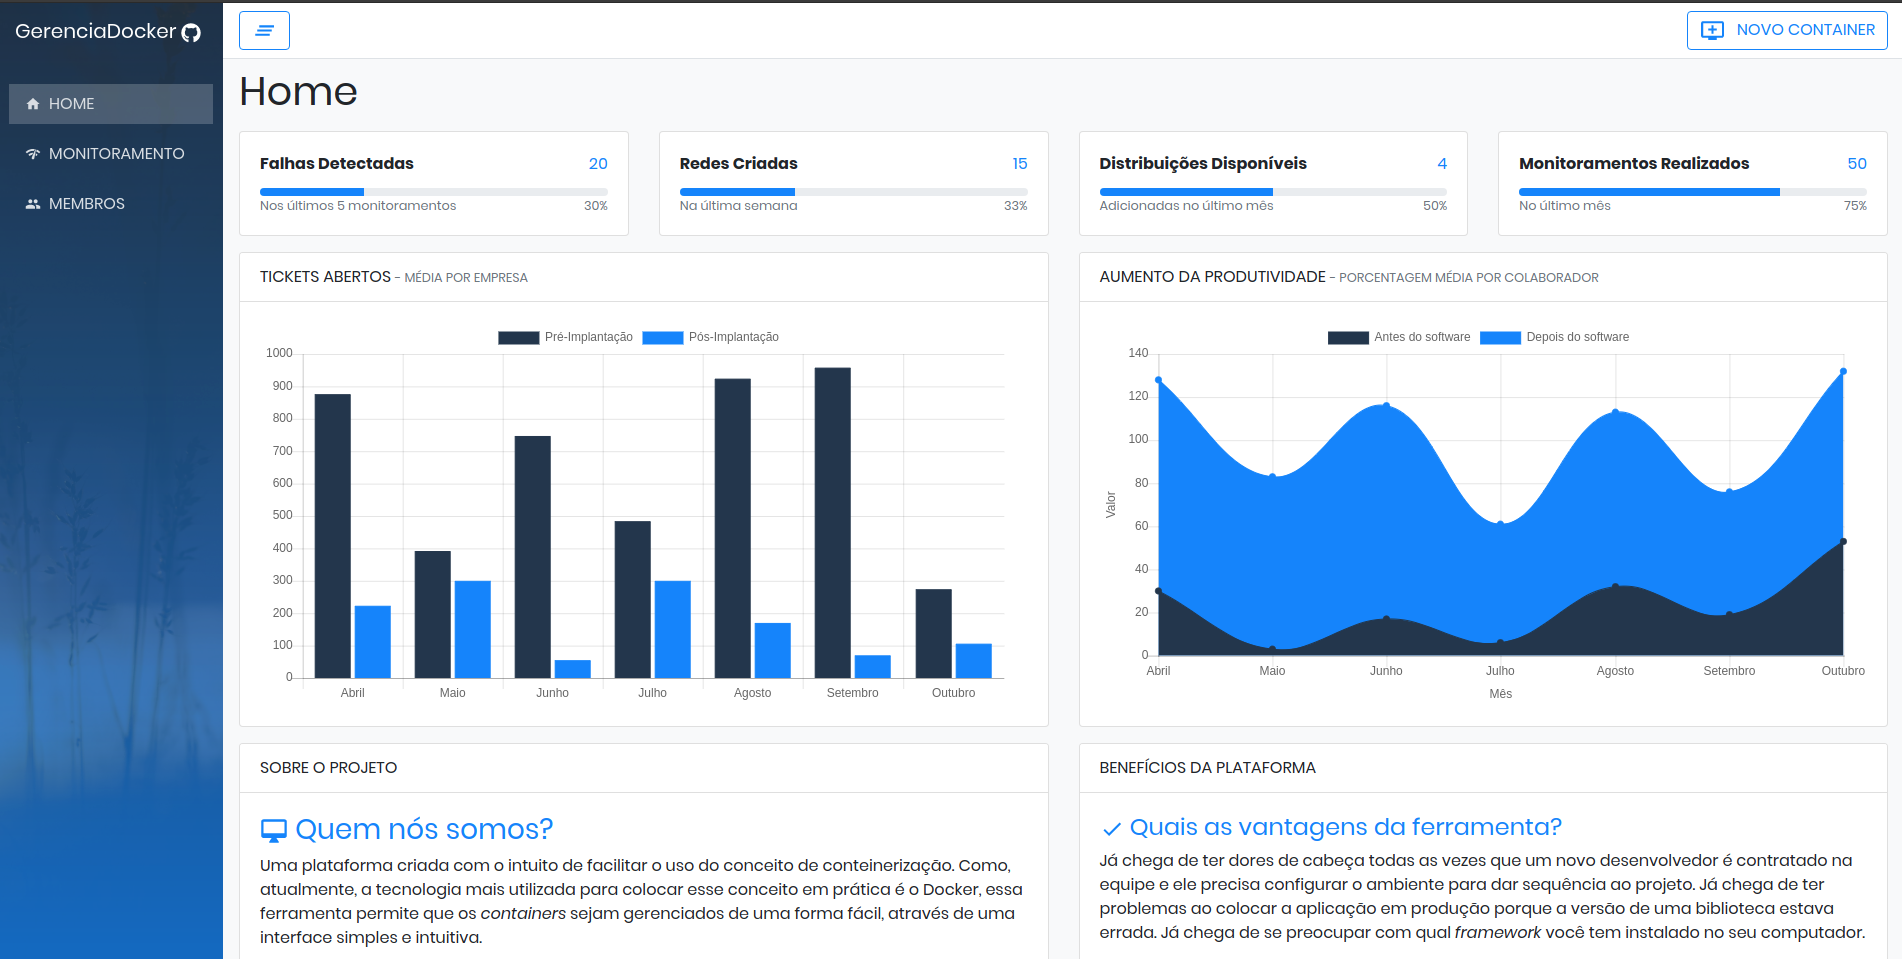
\includegraphics[width=1.0\textwidth]{./content/textuais/imagens/home-page.png}}
    \label{fig:home_page}
\end{figure}

Já a segunda, que é a tela de monitoramento, é o local mais importante do sistema e pode ser acessado através do menu lateral esquerdo. É nesse ambiente que o usuário criará sua \dockerNetwork{} e visualizará o estado atual de cada um dos \containers{} que a compõe. Além disso, também é possível interagir com cada \conteiner{} individualmente e utilizar opções como \aspas{Pausar}, \aspas{Retomar} ou \aspas{Excluir}, tal como pode ser visualizado na figura \ref{fig:monitoramento}.

\begin{figure}[!htb]
    \centering
    \caption{\textit{Monitoramento}}
    \frame{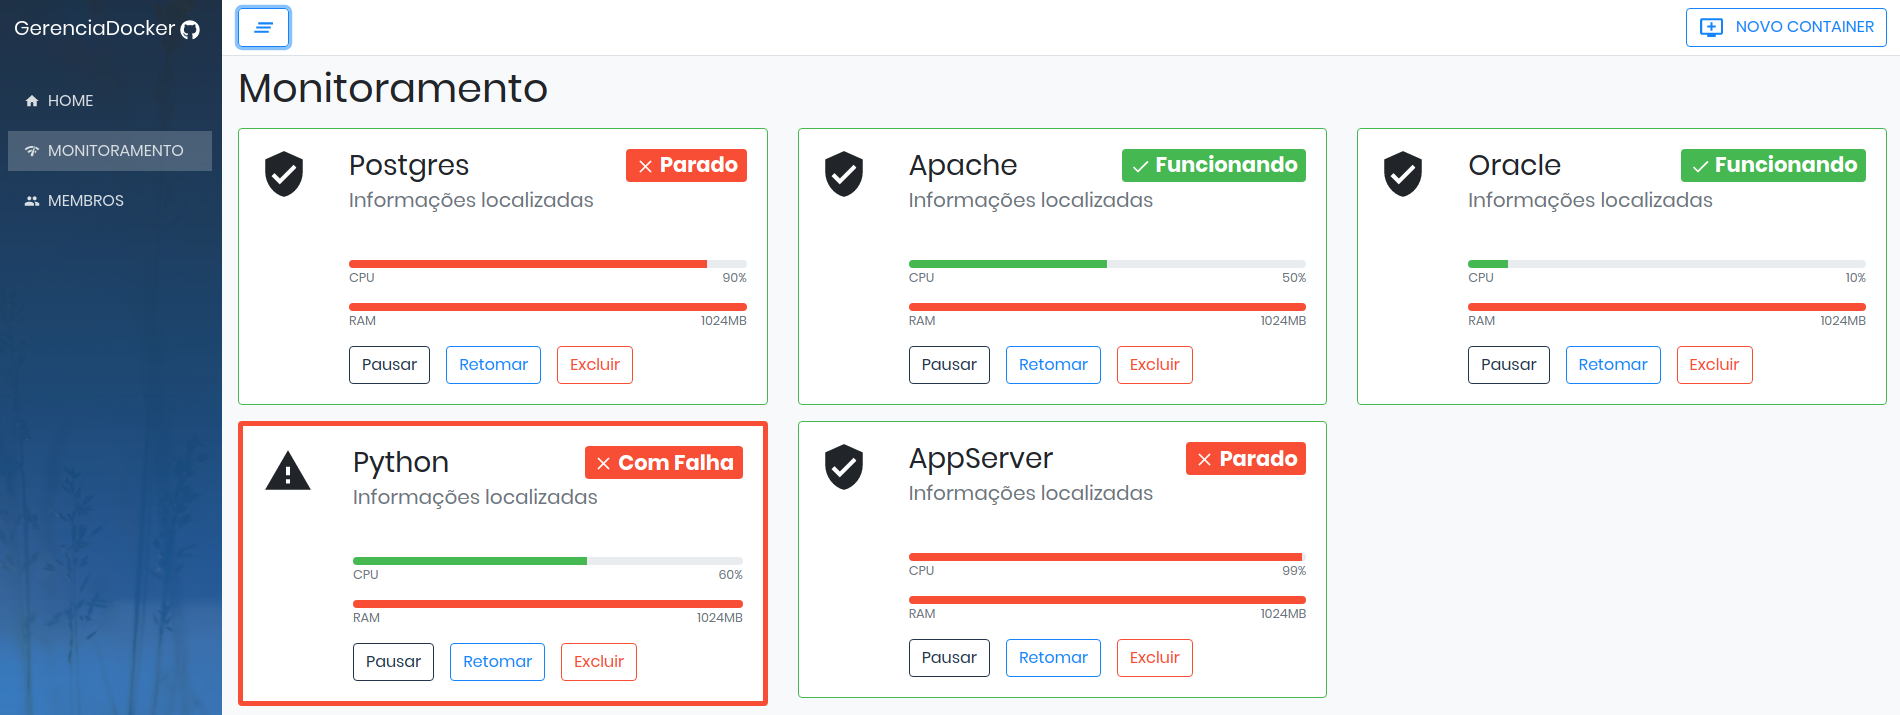
\includegraphics[width=1.0\textwidth]{./content/textuais/imagens/monitoring-page.png}}
    \label{fig:monitoramento}
\end{figure}

A principal funcionalidade utilizada na tela de monitoramento são os \textit{Hooks}, que permitem criar estados para armazenamento de dados e variáveis de forma rápida em uma função. Isto acelera o desenvolvimento, pois retira a necessidade da criação de classes para o funcionamento do \textit{front}.

Os \textit{Hooks} auxiliam o desenvolvedor a alcançar o principal objetivo do \textit{React}, que é fazer uma atualização dinâmica e prática dos componentes presentes na página, reduzindo o consumo de recursos e complexidade, pois abstraem conceitos e métodos para facilitar a construção da página.

% PWA-------------------------------------------------------------------
\section{PWA}
\label{sec:pwa}

Os \textit{Progressive Web Apps}, que recentemente vêm ganhando bastante popularidade e adeptos, podem ser definidos como \cite{Souza19} \aspas{uma aplicação \web{} com tecnologias que permitem termos a experiência de uso muito próxima da oferecida pelos \textit{mobile apps}}. Isso quer dizer, basicamente, que ao acessar um \textit{site}, o usuário terá a opção de adicionar um \aspas{atalho} para este no seu celular.

Porém, ao abrir esse atalho, a experiência para o usuário será de estar utilizando um aplicativo nativo, como se tivesse \aspas{instalado o \textit{site}} em seu dispositivo. Isso porque ele não verá uma barra exibindo a \textit{URL} que está sendo acessada e, além disso, funções nativas do celular - como acesso à câmera, geolocalização, aos contatos e \textit{push notifications} - estarão em pleno funcionamento. Esse tipo de solução tem sido testada e utilizada por grandes empresas como Uber, Twitter e Facebook, por exemplo, em virtude de algumas vantagens que ela apresenta sobre os \textit{apps} nativos, principalmente em dois pontos: custos e engajamento do cliente.


Primeiramente, no quesito despesas, utilizar um \textit{PWA} permite que, com poucas alterações no site da empresa, ela disponibilize um \aspas{aplicativo} - o que economiza tempo de desenvolvimento e, consequentemente, dinheiro. Em segundo lugar, geralmente os \textit{PWAs} são mais rápidos, ocupam menos espaço de armazenamento no dispositivo e, em casos reais, ficou comprovado que a facilidade em obter esse \textit{app} gera mais conversão de clientes, conforme \cite{Souza19} \aspas{o Flipkart que é o maior e-commerce da Índia, eles decidiram fazer uma experiência mobile através de uma PWA e aumentaram a sua conversão em 70\%}.

Para resumir, sempre que deseja-se criar uma experiência agradável para o usuário, de forma rápida e com poucos custos, não sendo necessário implementar funcionalidades demasiadamente robustas, um \textit{PWA} é a melhor opção. No caso desse projeto, portanto, que se enquadra perfeitamente nessas características, o grupo considerou essa como sendo a tecnologia ideal para criarmos um aplicativo.


\subsection{Desenvolvimento}
\label{subsec:desenvolvimento}

Após entender quais eram as tecnologias necessárias, realizar pesquisas sobre o assunto e realizar alguns cursos \online{}, pode-se dizer que o desenvolvimento do aplicativo não foi tão complexo - até porque sua funcionalidade é bastante simples. No entanto, como em qualquer outra aplicação, a curva de aprendizado inicial foi o obstáculo mais relevante que teve de ser superado. Após passar por esta etapa, trabalhou-se com foco na parte visual (procurando deixá-la agradável e responsiva) e nos testes do \textit{app}, pois um dos seus pontos mais atrativos é o envio de notificações e, portanto, era obrigatório que isso que estivesse funcionando corretamente. 

Ao fim da sua construção, pode-se dizer que esse aplicativo utilizou três recursos essenciais, sem os quais seu funcionamento seria inviável. Para que seja possível citar alguns detalhes técnicos, as seções a seguir serão destinadas especificamente a cada um deles: Firebase, GitHub e JavaScript.

\subsubsection{Firebase}
\label{subsubsec:firebase}

A plataforma, desenvolvida pela Google com o objetivo de tornar o desenvolvimento de aplicativos e sistemas mais fácil e rápida, é quem possibilita o envio das \textit{push notifications} pois, na realidade, é ela quem gerencia o envio e recebimento desses avisos. Isso porque, toda vez que a \textit{API} obter a informação de uma falha no container, ela enviará uma requisição \textit{POST} para um servidor do Firebase e, somente então, o Firebase irá reconhecer quem deve receber essa mensagem e a entregará ao seu destinatário final.

Além desse grande auxílio, a plataforma possui um console completamente focado em escalar exponencialmente qualquer tipo de solução que a utilize, tal como permitir a utilização de um banco de dados de tempo real em poucos \textit{clicks}. Essa grande variadade de ferramentas disponibilizadas pela mesma plataforma é um fato bastante positivo pois, caso o grupo decida evoluir ainda mais este projeto, diversos recursos atuais e de grande valia estariam disponíveis para serem utilizados facilmente.


\subsubsection{GitHub}
\label{subsubsec:github}

A plataforma de armazenamento de código teve dois papeis fundamentais para essa parte do projeto: o primeiro - e mais óbvio - é que o código foi versionado através da mesma, assim como os demais módulos da solução. No entanto, o segundo ponto é que a funcionalidade \textit{GitHub Pages} permitiu disponibilizar esse aplicativo \online{} e com um certificado HTTPS (requisito para o desenvolvimento de um \textit{PWA}). Com isso, foi possível hospedar o aplicativo e realizar a demonstração através da própria plataforma, como é possível ver na figura \ref{fig:github_pages}.

\begin{figure}[H]
    \centering
    \caption{\textit{GitHub Pages}}
    \frame{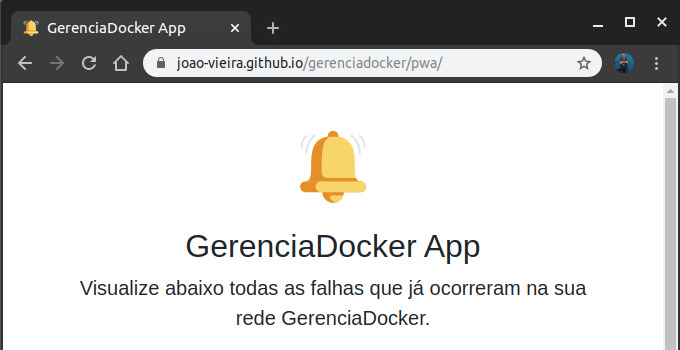
\includegraphics[width=1.0\textwidth]{./content/textuais/imagens/github_pages.png}}
    \label{fig:github_pages}
\end{figure}


\subsubsection{JavaScript}
\label{subsubsec:javascript}

É a linguagem de programação que foi utilizada para fazer todo o aplicativo. Além disso: é a responsável por criar os registros das falhas na tela dinamicamente, é nela que os \textit{Service Workers} são escritos (\textit{scripts} responsáveis por viabilizar o desenvolvimento das \textit{PWAs}), também é através dela que a comunicação com o \textit{firebase} é realizada e, por fim, é quem controla a inserção e leitura do \textit{localStorage} (mecanismo do navegador que permite o armazenamento de informações).

O trecho de código abaixo apresenta o registro do \textit{service worker}, que permite que o aplicativo seja utilizado mesmo sem conexão com a rede (\textit{off-line}):

\vspace*{1cm}
\begin{python}
    if ('serviceWorker' in navigator) {
        navigator.serviceWorker
            .register('service-worker.js')
            .then(reg => console.log("[ServiceWorker] Registered..."))
            [ . . .]
\end{python}
\vspace*{1cm}



\subsection{O Aplicativo}
\label{subsec:o_aplicativo}

Para tornar a solução ainda mais completa e próxima das necessidades do usuário, o grupo decidiu fazer um \textit{app} simples (utilizando a tecnologia citada no subcapítulo \ref{sec:pwa}) que irá listar todas as ocorrências de falhas nos \containers{}, além de disparar uma \textit{push notification} no dispositivo móvel do usuário. O objetivo principal deste aplicativo é servir como uma fonte de consulta para o usuário responsável pelo funcionamento da rede de \containers{}.

Isso porque, em virtude de relacionar-se com diversas variáveis (velocidade da rede, infraestrutura, tamanho das equipes, entre outras), é possível que esse tipo de rede apresente pequenas falhas com o decorrer do tempo. Como é de conhecimento de todos, o profissional moderno precisa, além de realizar várias tarefas em paralelo, contar com uma certa mobilidade e, portanto, não seria agradável que um colaborador precisasse monitorar a tela do sistema em tempo integral para identificar quando ocorresse um problema.

Em razão disso, era necessário chamar a atenção dos responsáveis por manter a rede funcionando de alguma forma. Analisando as tecnologias disponíveis nos dias de hoje, chegou-se ao consenso que uma notificação no celular é, provavelmente, um dos melhores meios de chamar a atenção de alguém. Na figura \ref{fig:aplicativo}, é possível visualizar a interface da versão final do aplicativo:

\begin{figure}[!htb]
    \centering
    \caption{Aplicativo}
    \frame{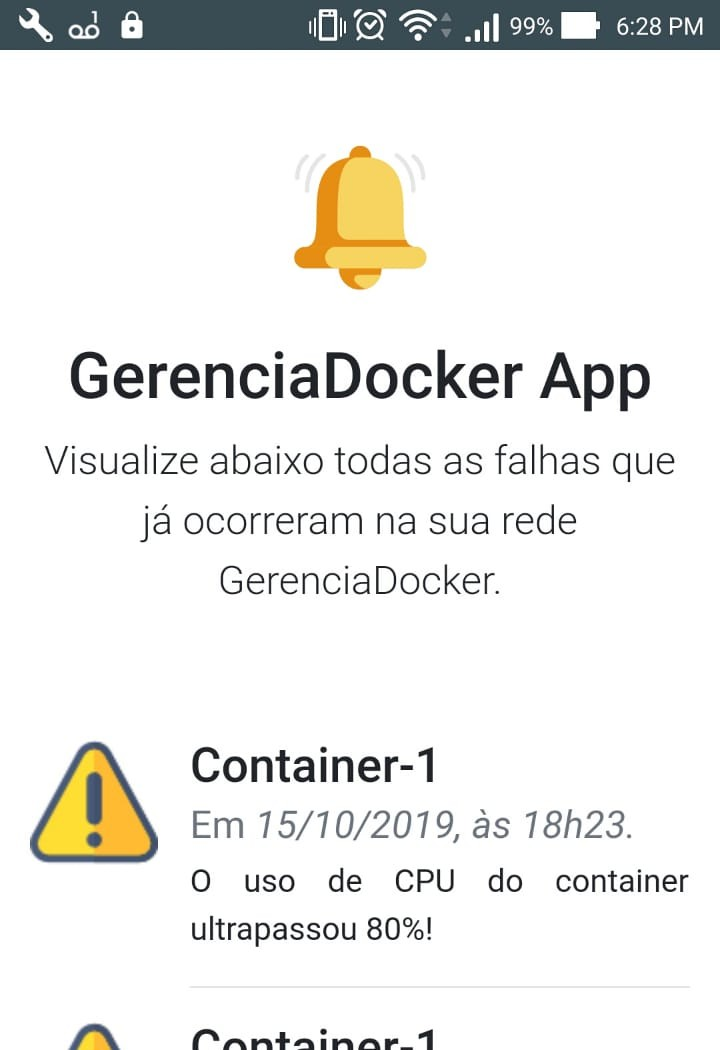
\includegraphics[width=0.4\textwidth]{./content/textuais/imagens/pwa.jpeg}}
    \label{fig:aplicativo}
\end{figure}